% The assembly design flow at a glance: the eight stages of
% docs/flow/01_overview.rst, grouped into three phases, with the artefact each
% phase hands to the next. Keep this in step with the stage table on that page.
\documentclass[border=2mm]{standalone}
\usepackage{tikz}
\usetikzlibrary{arrows.meta, positioning, calc, fit, backgrounds}
\usepackage[T1]{fontenc}
\usepackage{lmodern}

% Wrapped labels are short; break them at spaces only, never mid-word.
\hyphenpenalty=10000
\exhyphenpenalty=10000

\definecolor{IHPfg}{RGB}{0,80,139}
\definecolor{IHPaccent}{RGB}{109,112,114}
\definecolor{IHPgreen}{RGB}{65,155,75}
\definecolor{cChiplet}{RGB}{55,145,195}

\begin{document}
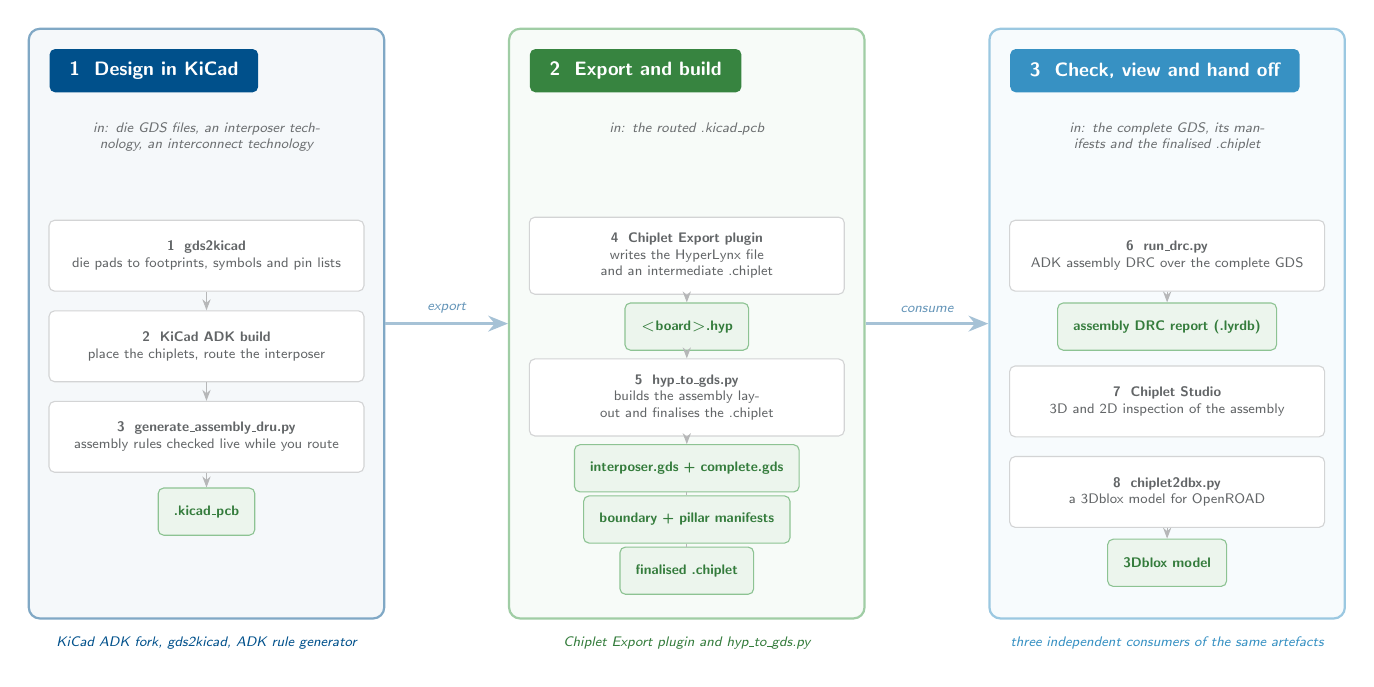
\begin{tikzpicture}[
    >=Stealth,
    adkstep/.style={
        rectangle, rounded corners=2pt,
        draw=IHPaccent!30, fill=white, line width=0.4pt,
        text width=36mm, minimum height=9mm,
        font=\sffamily\tiny, text=IHPaccent!90!black, align=center, inner sep=2mm
    },
    adkout/.style={
        rectangle, rounded corners=2pt,
        draw=IHPgreen!60, fill=IHPgreen!10, line width=0.4pt,
        minimum height=6mm, inner xsep=2mm,
        font=\sffamily\tiny\bfseries, text=IHPgreen!80!black
    },
    adkin/.style={
        text width=36mm, align=center, inner sep=0pt,
        font=\sffamily\tiny\itshape, text=IHPaccent
    },
    pbox/.style={
        rectangle, rounded corners=4pt,
        draw=#1!50, fill=#1!4, line width=0.8pt,
        inner xsep=2.5mm, inner ysep=2.5mm
    },
    ptitle/.style={
        rectangle, rounded corners=2pt,
        fill=#1, font=\sffamily\scriptsize\bfseries, text=white,
        minimum height=5.5mm, inner xsep=2.5mm
    },
    tlbl/.style={font=\sffamily\fontsize{4.5}{5.5}\selectfont\itshape, text=#1},
    pad/.style={inner sep=0pt, minimum size=0pt},
    arr/.style={-{Stealth[length=1.4mm]}, line width=0.35pt, color=IHPaccent!50},
    lnk/.style={line width=0.35pt, color=IHPaccent!50},
    bigarr/.style={-{Stealth[length=2.5mm, width=2mm]}, line width=1.2pt, color=IHPfg!35}
]

% ========== PHASE 1: design in KiCad (stages 1 to 3) ==========

\node[ptitle=IHPfg, anchor=west] (t1) at (-8.1, 0) {1 ~Design in KiCad};

\node[adkin, anchor=north] (i1) at (-6.1, -0.65)
    {in: die GDS files, an interposer technology, an interconnect technology};

\node[adkstep] (s1) at (-6.1, -2.35)
    {\textbf{1 ~gds2kicad}\\die pads to footprints, symbols and pin lists};
\node[adkstep] (s2) at (-6.1, -3.50)
    {\textbf{2 ~KiCad ADK build}\\place the chiplets, route the interposer};
\node[adkstep] (s3) at (-6.1, -4.65)
    {\textbf{3 ~generate\_assembly\_dru.py}\\assembly rules checked live while you route};
\node[adkout] (o1) at (-6.1, -5.60) {.kicad\_pcb};
\node[pad] (b1) at (-6.1, -6.70) {};

\draw[arr] (s1) -- (s2);
\draw[arr] (s2) -- (s3);
\draw[arr] (s3) -- (o1);

\begin{pgfonlayer}{background}
  \node[pbox=IHPfg, fit=(t1)(i1)(s1)(s2)(s3)(o1)(b1)] (p1) {};
\end{pgfonlayer}
\node[tlbl=IHPfg, anchor=north] at ([yshift=-1mm]p1.south)
    {KiCad ADK fork, gds2kicad, ADK rule generator};

% ========== PHASE 2: export and build (stages 4 and 5) ==========

\node[ptitle=IHPgreen!85!black, anchor=west] (t2) at (-2.0, 0) {2 ~Export and build};

\node[adkin, anchor=north] (i2) at (0, -0.65)
    {in: the routed .kicad\_pcb};

\node[adkstep] (h1) at (0, -2.35)
    {\textbf{4 ~Chiplet Export plugin}\\writes the HyperLynx file and an intermediate .chiplet};
\node[adkout] (o2a) at (0, -3.25) {\textless{}board\textgreater{}.hyp};
\node[adkstep] (h2) at (0, -4.15)
    {\textbf{5 ~hyp\_to\_gds.py}\\builds the assembly layout and finalises the .chiplet};
\node[adkout] (o2b) at (0, -5.05) {interposer.gds + complete.gds};
\node[adkout] (o2c) at (0, -5.70) {boundary + pillar manifests};
\node[adkout] (o2d) at (0, -6.35) {finalised .chiplet};
\node[pad] (b2) at (0, -6.70) {};

\draw[arr] (h1) -- (o2a);
\draw[arr] (o2a) -- (h2);
\draw[arr] (h2) -- (o2b);
\draw[lnk] (o2b) -- (o2c);
\draw[lnk] (o2c) -- (o2d);

\begin{pgfonlayer}{background}
  \node[pbox=IHPgreen, fit=(t2)(i2)(h1)(o2a)(h2)(o2b)(o2c)(o2d)(b2)] (p2) {};
\end{pgfonlayer}
\node[tlbl=IHPgreen!80!black, anchor=north] at ([yshift=-1mm]p2.south)
    {Chiplet Export plugin and hyp\_to\_gds.py};

% ========== PHASE 3: check, view and hand off (stages 6 to 8) ==========

\node[ptitle=cChiplet, anchor=west] (t3) at (4.1, 0) {3 ~Check, view and hand off};

\node[adkin, anchor=north] (i3) at (6.1, -0.65)
    {in: the complete GDS, its manifests and the finalised .chiplet};

\node[adkstep] (v1) at (6.1, -2.35)
    {\textbf{6 ~run\_drc.py}\\ADK assembly DRC over the complete GDS};
\node[adkout] (o3a) at (6.1, -3.25) {assembly DRC report (.lyrdb)};
\node[adkstep] (v2) at (6.1, -4.20)
    {\textbf{7 ~Chiplet Studio}\\3D and 2D inspection of the assembly};
\node[adkstep] (v3) at (6.1, -5.35)
    {\textbf{8 ~chiplet2dbx.py}\\a 3Dblox model for OpenROAD};
\node[adkout] (o3b) at (6.1, -6.25) {3Dblox model};
\node[pad] (b3) at (6.1, -6.70) {};

\draw[arr] (v1) -- (o3a);
\draw[arr] (v3) -- (o3b);

\begin{pgfonlayer}{background}
  \node[pbox=cChiplet, fit=(t3)(i3)(v1)(o3a)(v2)(v3)(o3b)(b3)] (p3) {};
\end{pgfonlayer}
\node[tlbl=cChiplet, anchor=north] at ([yshift=-1mm]p3.south)
    {three independent consumers of the same artefacts};

% ========== phase to phase ==========

\draw[bigarr] (p1.east) -- node[tlbl=IHPfg!60, above] {export} (p2.west);
\draw[bigarr] (p2.east) -- node[tlbl=IHPfg!60, above] {consume} (p3.west);

\end{tikzpicture}
\end{document}
